\documentclass[a4paper,10pt]{report}
\usepackage[T1]{fontenc}
\usepackage{mathptmx}
\usepackage{graphicx}
\graphicspath{ {Diagrams/} }

\title{Assignment 3.2 documentation}

\author{Péter Zaváczki\\30433}

\begin{document}

\maketitle

\section{Requirements}
Design, implement and test a distributed system that uses MOM to create an asynchronous
communication between the client (message producer) and the server (message consumer). 

\section{Functional requirements}
\begin{itemize}
    \item The application is used by a DVD store administrator
    \item The administrator must send notification to its customers when a new DVD is available
    \item The information about the new DVD must be saved in a text file
    \item Each time new information about a DVD is introduced in the system, the application must send automatically notification e-mails to all the subscriber customers to notify them about the new item
    \item Each time new information about a DVD is introduced in the system the application must create automatically a text file and write the information about the DVD in it    
\end{itemize}

\section{Implementation technologies}
\begin{itemize}
    \item For message producer and consumer: Java
    \item For message queue: Java: JMS, Java API of RabbitMQ
\end{itemize}

\section{Conceptual architecture}
This application has a complex architecture. It has a Client-Server component which is the webapp, in this case the Client being the user's web browser, to which the webpages are loaded and the server is the Tomcat server to which the WAR files are deployed.
The message transmission is done using a MOM, RabbitMQ. The MOM's producer is connected to the webapp's servlet to take the information. The producer serializes the POJO which was constructed using the data received from the POST request and the resulting byte array is put into the MOM's queue. The consumer takes the messages, it deserializes these byte arrays back into a POJO and further handles them by sending emails and saving it to a text file.

This can be seen on figure \ref{fig:architecture_diagram}.

\begin{figure}[h]
    \centering
    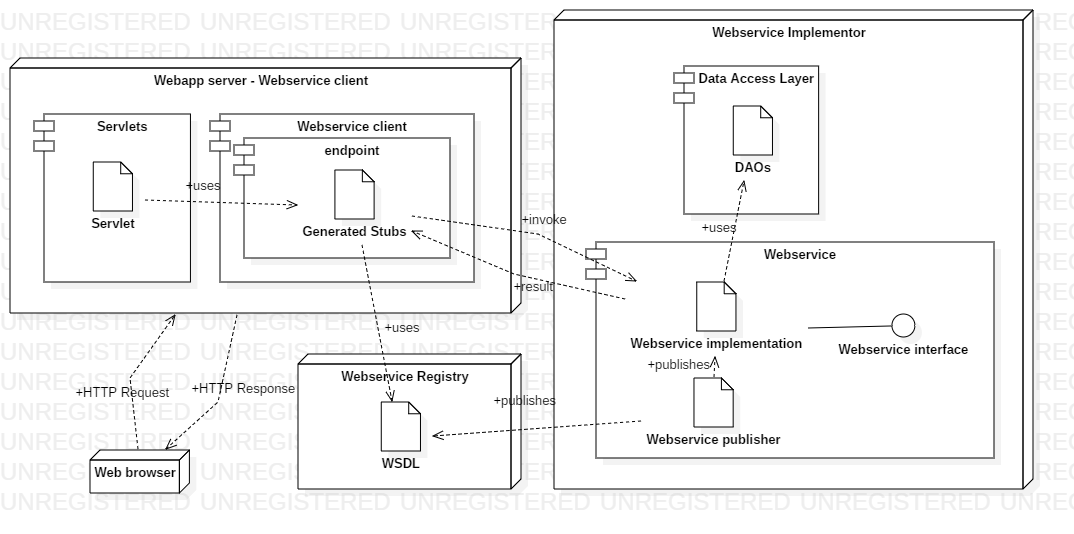
\includegraphics[width=1\textwidth]{architecture_diagram.png}
    \caption{The conceptual architecture diagram of the project}
    \label{fig:architecture_diagram}
\end{figure}

\section{Deployment}
The application is deployed on multiple nodes:
The webapp is deployed on a Tomcat server, which has the Web Application Resource (WAR) files.
The messages are transferred using a Message-Oriented Middleware (MOM), RabbitMQ. This has a message queue, to which the message producer adds messages to be later consumed by the receiver.

This deployment can be seen on figure \ref{fig:deployment_diagram}.

\begin{figure}[h]
    \centering
    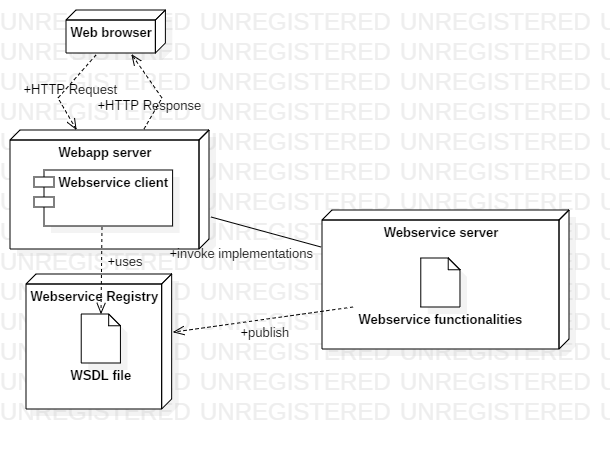
\includegraphics[width=1\textwidth]{deployment_diagram.png}
    \caption{The deployment diagram of the project}
    \label{fig:deployment_diagram}
\end{figure}

\section{Build considerations}
\begin{itemize}
    \item Java Message Service (JMS) was used instead of Microsoft Message Queueing (MSMQ), due to the programming language chosen to implement the assignment with.
\end{itemize}


\end{document}
